\documentclass[11pt]{article}

% Use the official ACL style package from https://github.com/acl-org/acl-style-files.
% Place acl.sty and acl_natbib.bst next to this file when compiling outside an
% existing ACL/Overleaf template.
\usepackage[preprint]{acl}

\usepackage{times}
\usepackage{latexsym}
\usepackage[T1]{fontenc}
\usepackage[utf8]{inputenc}
\usepackage{microtype}
\usepackage{inconsolata}
\usepackage{graphicx}
\usepackage{booktabs}
\usepackage{array}
\usepackage{xcolor}
\usepackage{url}

\title{BabyActionLM: Can BabyLM-Scale Models Learn Mobile Tool-Call Parsing?}

\author{
Pragnesh Kumar Pallaprolu \\
Neural Networks for NLP \\
\texttt{BabyActionLM course project}
}

\begin{document}
\maketitle

\begin{abstract}
BabyActionLM studies whether very small BabyLM-style causal language models can learn a narrow mobile-agent skill: mapping natural-language phone commands to structured tool calls. The project is an NLP parsing experiment on the simulated \texttt{google/mobile-actions} dataset, not an Android app. I fine-tune two course checkpoints, BabyA and BabyB, on 8,693 Mobile Actions training examples and evaluate on the official 961-example evaluation subset. I compare them with zero-shot \texttt{functiongemma:270m}, a local function-calling model, using parse rate, function accuracy, argument exact match, and full tool-call exact match. BabyB improves substantially over BabyA with compact JSON targets, reaching 35.6\% parse rate and 5.3\% function accuracy, but both Baby models obtain 0 full exact matches. A flatter domain-specific language (DSL) target gives BabyB only a tiny exact-match signal of 0.7\%. FunctionGemma is much stronger, reaching 49.6\% exact match. These results suggest that stronger BabyLM-style pretraining helps tiny models move toward structured action parsing, but this setup is not reliable enough for a local phone controller.

\end{abstract}

\section{Introduction}

Modern assistants increasingly expose tool-calling interfaces: a user request is converted into a structured function name and arguments, and another system executes the action. On mobile devices, this framing is attractive because many commands are simple and private: create a contact, schedule an event, send an email, open Wi-Fi settings, toggle the flashlight, or show a place on a map. A very small local model would be useful if it could parse these requests without contacting a large cloud model.

BabyActionLM asks a narrower scientific question: can BabyLM-scale pretraining help a tiny neural language model learn simulated mobile tool-call parsing? The experiment does not execute actions on an Android phone. Instead, it treats the phone as a fixed tool schema and studies language-to-structure prediction with neural causal language models.

The main comparison is between two course checkpoints, BabyA and BabyB, fine-tuned with the same Mobile Actions data and evaluation pipeline. BabyB represents the stronger BabyLM-style pretrained model. I also include \texttt{functiongemma:270m}, evaluated zero-shot through Ollama native tool calling, as a practical local function-calling reference. It is not a same-size baseline; rather, it shows what a model designed for function calling can do on the same examples.

The results are mixed but informative. With compact JSON targets, BabyB is clearly stronger than BabyA: parse rate rises from 1.9\% to 35.6\%, and function accuracy rises from 0.3\% to 5.3\%. However, both Baby models fail exact tool-call matching in this setting. I also test a flatter DSL target to check whether the weakness is mainly serialization. It produces a small nonzero exact-match signal for BabyB, 0.7\%, but lowers parse and function accuracy compared with the JSON target. FunctionGemma remains far ahead with 98.1\% parse rate and 49.6\% exact tool-call match.

The contribution of this report is therefore not a deployable phone controller. It is a compact controlled experiment showing that BabyLM-scale pretraining can improve a tiny model's structured parsing behavior, while also showing that simple causal-LM fine-tuning with a 128-token context is not enough for reliable mobile action control.

\section{Background and Related Work}

\paragraph{BabyLM-scale modeling.}
The BabyLM framing asks how much linguistic behavior can be learned under small, developmentally inspired data and model budgets. The GPT-wee paper by \citet{bunzeck-zarriess-2023-gpt} studies very small GPT-style language models in this setting. BabyActionLM uses the same broad motivation in a downstream structured prediction task: rather than evaluating general linguistic fluency, it asks whether course BabyLM checkpoints can be adapted to a narrow action-parsing interface.

\paragraph{Tool use as language modeling.}
Toolformer frames tool use as a language-modeling problem in which a model learns when to call external APIs and what arguments to pass \citep{schick-etal-2023-toolformer}. BabyActionLM removes the harder multi-step setting and focuses on one decision: given a command and available phone tools, generate one structured call.

\paragraph{Small function-calling agents.}
TinyAgent shows that task-specific smaller language models can be trained for function calling and deployed at the edge \citep{erdogan-etal-2024-tinyagent}. FunctionGemma is a small Gemma-family model variant intended for function-calling workflows \citep{google-functiongemma}, and Ollama provides a local \texttt{functiongemma:270m} package with native tool-call examples and benchmark notes \citep{ollama-functiongemma}. BabyActionLM is smaller in scope: it uses BabyA/B course checkpoints and a simulated phone-action dataset to test whether very small models can learn the basic language-to-tool-call mapping.

\section{Task and Dataset}

The task is single-step mobile tool-call parsing. Each example contains a developer message with the available tool context, a user command, and an assistant tool call. The target is normalized to a canonical schema:

\begin{center}
\small
\texttt{\{"name": tool, "arguments": \{...\}\}}
\end{center}

I use \texttt{google/mobile-actions}, a public Hugging Face dataset for mobile assistant function calls \citep{google-mobile-actions}. Hugging Face exposes the data as one split, but the rows contain a metadata field that separates 8,693 training examples from 961 evaluation examples. The report uses that official metadata split throughout.

The tool inventory contains seven phone-style actions: \texttt{create\_calendar\_event}, \texttt{create\_contact}, \texttt{open\_wifi\_settings}, \texttt{send\_email}, \texttt{show\_map}, \texttt{turn\_off\_flashlight}, and \texttt{turn\_on\_flashlight}. Arguments vary from empty dictionaries for flashlight commands to multiple fields for contact, email, calendar, and map commands.

Because BabyA and BabyB have a 128-token context window, the prompt is compressed. It contains a short task instruction, semicolon-separated tool signatures, the user command, and a generation marker. The main target format is compact JSON. I also test a flatter DSL target, such as:

\begin{center}
\small
\texttt{tool=show\_map;query=Rijksmuseum in Amsterdam}
\end{center}

Both target formats are parsed back into the same canonical tool-call object before scoring, so the evaluation metrics remain comparable.

\section{Models and Method}

\paragraph{BabyA and BabyB.}
BabyA and BabyB are tiny LLaMA-style causal language model checkpoints from the course assignment artifacts. Both are fine-tuned as sequence-to-sequence behavior through causal language modeling: the model receives the prompt plus target, and the loss is applied only to target tokens. BabyA and BabyB use the same formatting, split, optimizer settings, and evaluation scripts. This makes their comparison a test of whether the stronger BabyLM-style pretraining represented by BabyB transfers better to mobile action parsing.

\paragraph{FunctionGemma reference.}
\texttt{functiongemma:270m} is evaluated zero-shot through Ollama native tool calling. The same Mobile Actions tool schemas are normalized for Ollama, predictions are converted into the shared internal tool-call schema, and metrics are computed by the same scoring code. This baseline is stronger and larger than the Baby models and is treated as a practical local reference point, not as a same-size control.

\paragraph{Metrics.}
I report four metrics. Parse rate measures whether the generated output can be parsed into the canonical schema. Function accuracy measures whether the predicted function name equals the gold function name, over all examples. Argument exact match requires the complete argument dictionary to match after normalization. Tool-call exact match requires both the function and all arguments to match. This separation is important because a tiny model can learn a tool family without copying the correct argument span.

\paragraph{Format diagnostic.}
The compact JSON results suggested that syntax and nested structure might be a major failure point. I therefore compare JSON and DSL targets for BabyB on a held-out development split drawn only from the training rows. The official 961-example evaluation subset is untouched until final reporting.

\section{Experiments}

For the main JSON experiment, BabyA and BabyB are fine-tuned for three epochs on all 8,693 training examples and evaluated on all 961 official evaluation examples. Training uses conservative local-GPU settings: compact 128-token examples, small batches, gradient accumulation, and half precision when CUDA is available. Raw model outputs and checkpoints are kept outside the tracked report artifacts; the paper uses the tracked CSV summaries and figures under \texttt{results/}.

For the format diagnostic, BabyB is used for model-selection trials on a development subset of the training data. Four variants are compared: JSON for 3 epochs, JSON for 8 epochs, DSL for 3 epochs, and DSL for 8 epochs. Selection prioritizes exact tool-call match, then function accuracy, then parse rate. The selected variant is the 3-epoch DSL setup because it is the only development trial with nonzero exact match. BabyA and BabyB are then evaluated with this selected DSL setup on the official evaluation subset.

FunctionGemma is evaluated zero-shot on the same 961 examples. It receives the tool schema through Ollama's tool-calling interface and is not fine-tuned on Mobile Actions. All systems are scored with the same parser and metric implementation.

\section{Results and Analysis}

\begin{table*}[t]
\centering
\small
\begin{tabular}{lrrrr}
\toprule
Model & Parse & Function & Arguments & Exact Call \\
\midrule
BabyA JSON & 0.0187 & 0.0031 & 0.0000 & 0.0000 \\
BabyB JSON & 0.3559 & 0.0531 & 0.0000 & 0.0000 \\
FunctionGemma 270M & 0.9813 & 0.7097 & 0.5099 & 0.4964 \\
BabyA DSL & 0.3632 & 0.0000 & 0.0937 & 0.0000 \\
BabyB DSL & 0.1145 & 0.0083 & 0.0250 & 0.0073 \\
\bottomrule
\end{tabular}
\caption{Official Mobile Actions evaluation results on 961 examples. Exact call requires both function name and full argument dictionary to match.}
\label{tab:main-results}
\end{table*}

Table~\ref{tab:main-results} gives the main result. BabyB is much better than BabyA under the same JSON setup, especially on parse rate and function accuracy. This supports the central pretraining hypothesis in a limited comparative sense: the stronger Baby model moves closer to structured parsing. However, the task remains unsolved for both Baby models. BabyB often produces parseable JSON fragments, but it does not produce exact full tool calls.

\begin{figure}[t]
\centering
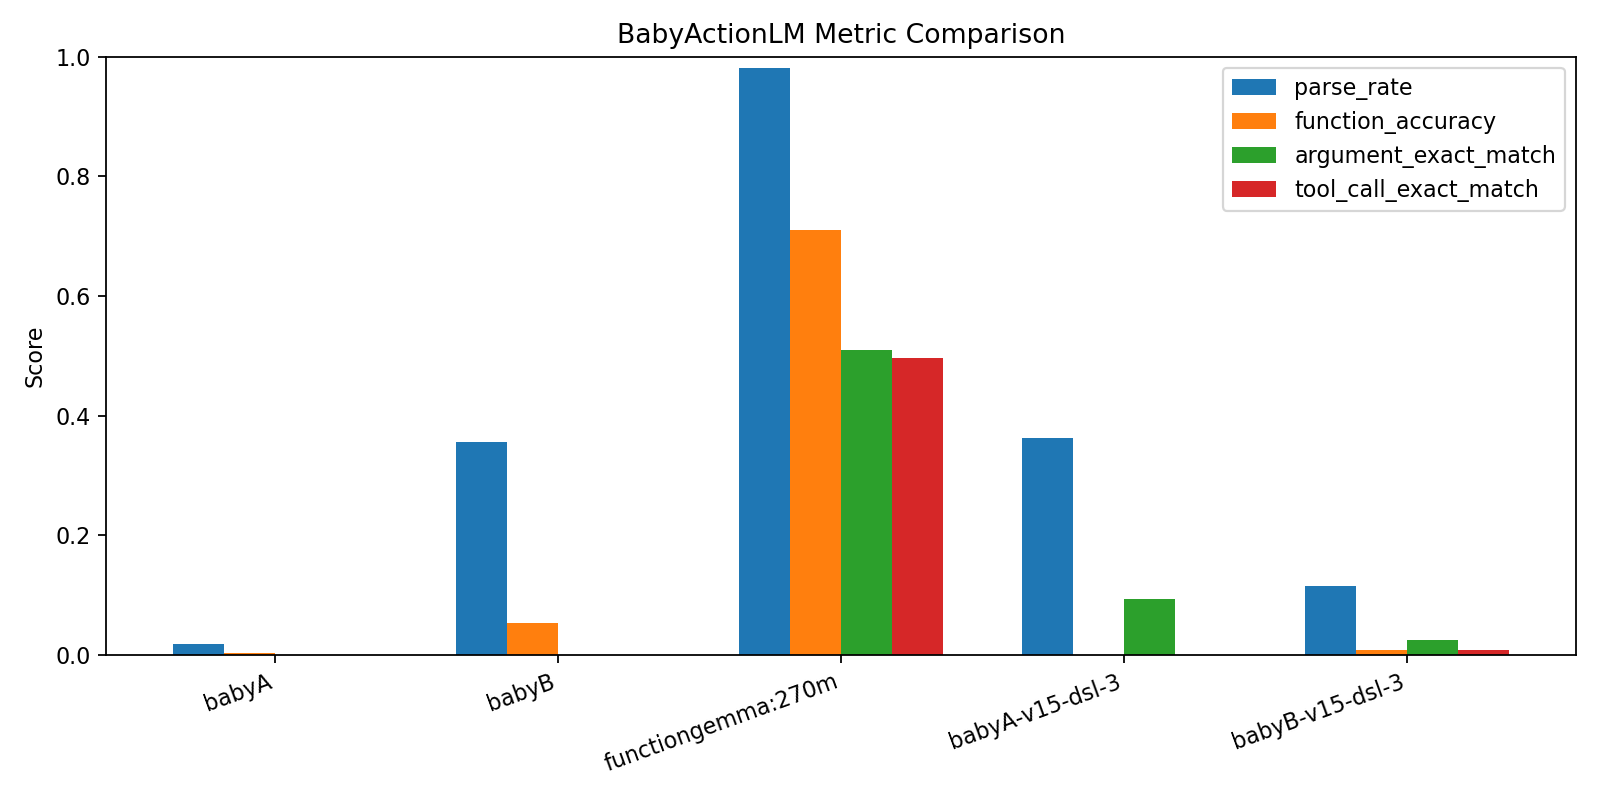
\includegraphics[width=\columnwidth]{figures/metric_comparison.png}
\caption{Metric comparison across BabyA, BabyB, the DSL diagnostic runs, and FunctionGemma.}
\label{fig:metrics}
\end{figure}

Figure~\ref{fig:metrics} highlights the gap between the fine-tuned Baby checkpoints and FunctionGemma. FunctionGemma reaches 98.1\% parse rate and 49.6\% exact tool-call match. This shows that the dataset and metric are meaningful: the task is not impossible, but it is far beyond what the current BabyA/B fine-tuning setup can reliably solve.

\begin{figure}[t]
\centering
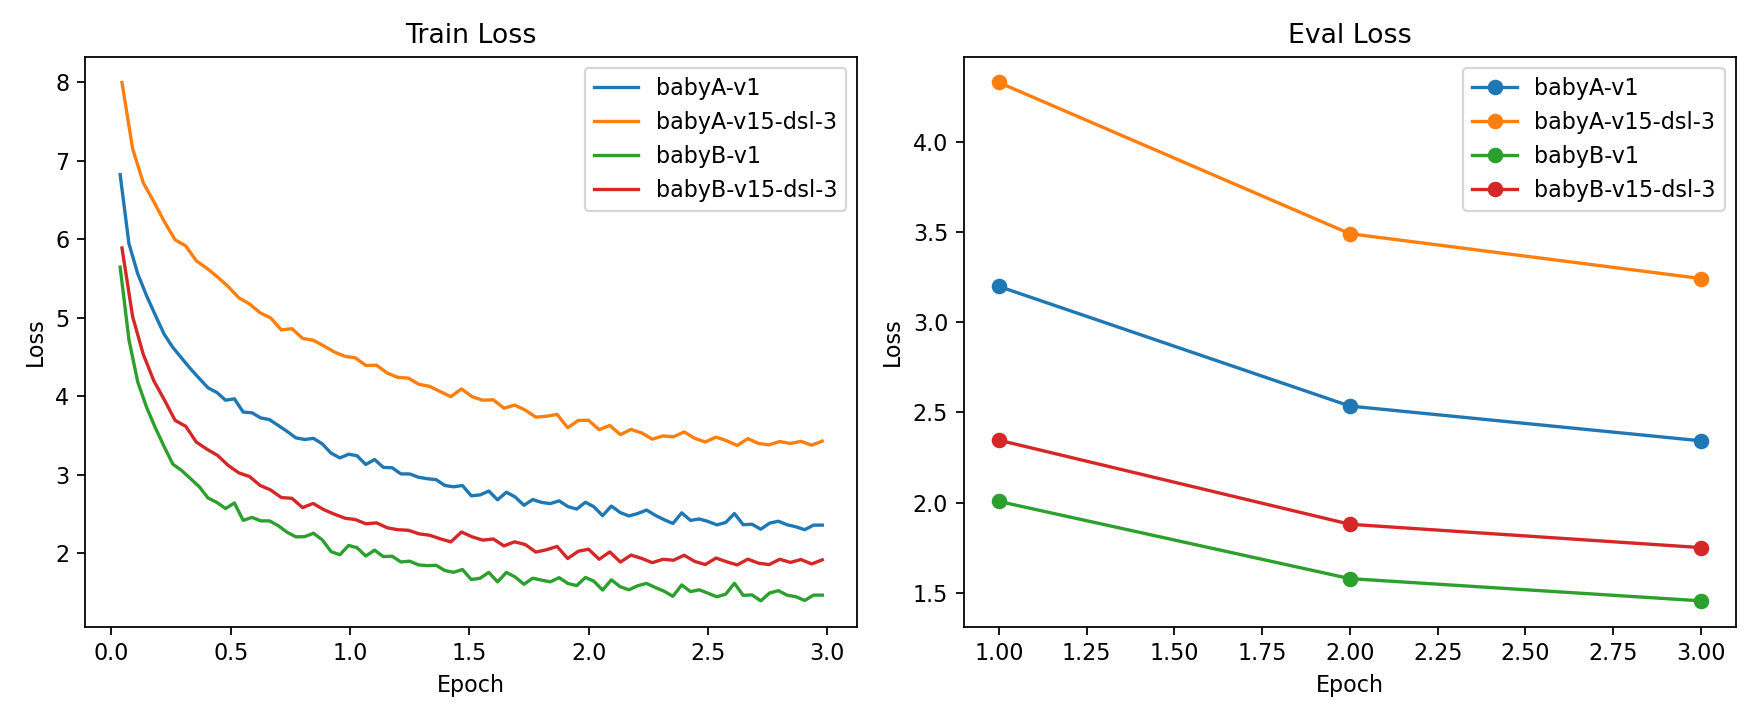
\includegraphics[width=\columnwidth]{figures/training_curves.png}
\caption{Fine-tuning loss curves for JSON and selected DSL BabyA/B runs. BabyB reaches lower evaluation loss than BabyA, but lower loss does not imply reliable exact tool calls.}
\label{fig:training}
\end{figure}

The training curves in Figure~\ref{fig:training} provide another view of the BabyA/B difference. BabyB reaches lower evaluation loss than BabyA in both target formats. This is consistent with the metric advantage in Table~\ref{tab:main-results}, but also shows the limit of token-level training loss as a proxy for structured correctness: exact arguments remain fragile even when loss decreases.

\paragraph{Format sensitivity.}
The format-selection trial gives partial support to the output-format hypothesis. On the BabyB development split, the 3-epoch DSL setup is the only variant with nonzero exact match, 0.0080, while the longer JSON run has better parse and function scores but still 0 exact match. On official eval, BabyB with the selected DSL target reaches 0.0073 exact match. This is a real but tiny signal. The honest interpretation is that target format matters, but a flatter string format does not solve mobile tool-call parsing for these models. BabyA with the same DSL target is especially cautionary: it reaches 36.3\% parse rate but 0 function accuracy, so parseability alone is not semantic success.

\paragraph{Per-tool behavior.}
The per-tool results show that BabyB's JSON function accuracy is concentrated in \texttt{show\_map}: 34.5\% function accuracy for that tool, while the other tools are effectively 0. FunctionGemma is strong across simple tools, especially flashlight and Wi-Fi actions, but argument-heavy tools such as contact creation and email remain harder. This suggests that copying or normalizing arguments is a separate challenge from choosing the action type.

\begin{table}[t]
\centering
\small
\begin{tabular}{p{0.28\columnwidth}p{0.62\columnwidth}}
\toprule
Field & Text \\
\midrule
Command & Show the location of the Rijksmuseum in Amsterdam on the map. \\
Gold & Tool: \texttt{show\_map}; query: Rijksmuseum in Amsterdam. \\
BabyB JSON & Tool: \texttt{show\_map}; query: \texttt{mail-020-101-10t10:00:00}. \\
\bottomrule
\end{tabular}
\caption{Qualitative BabyB example. The tool name is correct, but the argument is unrelated to the command.}
\label{tab:qual}
\end{table}

Table~\ref{tab:qual} shows the common partial-learning pattern. BabyB identifies that a location request should call \texttt{show\_map}, but it fails to copy the requested location into the argument. This explains why function accuracy can improve while argument exact match remains 0.

\section{Limitations and Conclusion}

This project has several limitations. First, it is simulated tool-call parsing, not real phone automation. The results say whether a model can emit a structured call from a dataset example; they do not measure latency, safety, UI grounding, permission handling, or execution on Android. Second, BabyA and BabyB are compared with each other, but there is no randomly initialized scratch control in the final experiment. Therefore the report can say that BabyB's stronger pretraining appears helpful relative to BabyA, but it cannot prove pretraining is the only cause of the difference. Third, the 128-token context forces compressed prompts and tool signatures, which may make the task harder than it would be for a larger model or a classifier-style architecture.

The final conclusion is deliberately modest. BabyLM-style pretraining helps tiny models move toward structured mobile action parsing: BabyB learns more parseable outputs and more correct function names than BabyA under identical fine-tuning. But BabyA/B are not reliable local phone controllers in this setup. The DSL diagnostic shows that serialization format can create a tiny exact-match signal, while FunctionGemma shows that a small model designed for function calling can solve many more examples on the same evaluation set. BabyActionLM therefore demonstrates both the promise and the current limitation of very small neural language models for local tool-call parsing.


\bibliography{references/references}

\end{document}
